	\section{\textbf{Acelerómetro}}
	Un acelerómetro es un sensor diseñado para medir la aceleración de un objeto, es decir, la variación de su velocidad en función del tiempo. Además de cuantificar la aceleración, estos dispositivos pueden determinar la velocidad y el desplazamiento mediante la integración de la señal de aceleración. Son fundamentales en aplicaciones que requieren monitoreo de vibraciones, análisis de movimiento y detección de impactos.
\subsection{\textbf{Tipos de Acelerómetros}}
\subsubsection{\textbf{Acelerómetros Piezoeléctricos}}
Utilizan materiales piezoeléctricos que generan una carga eléctrica proporcional a la fuerza de aceleración aplicada. Son ideales para mediciones dinámicas debido a su amplio rango de frecuencia y estabilidad a largo plazo. Sin embargo, no pueden medir aceleraciones estáticas o de muy baja frecuencia.

\subsubsection{\textbf{Acelerómetros MEMS (Sistemas Microelectromecánicos)}}
Estos dispositivos están acoplados a corriente continua (CC) y pueden responder a frecuencias tan bajas como 0 Hz, permitiendo la medición de aceleraciones estáticas o de frecuencia muy baja. Son comunes en aplicaciones de monitoreo de condiciones y mantenimiento predictivo.

\subsubsection{\textbf{Acelerómetros Piezorresistivos}}
Funcionan basándose en cambios de resistencia en galgas extensométricas cuando se aplica una aceleración. Son adecuados para medir aceleraciones de alta magnitud y ofrecen un amplio ancho de banda, siendo útiles en aplicaciones como pruebas de choque y seguridad automotriz.

\subsection{\textbf{¿Cómo Funciona un Acelerómetro?}}
El principio de funcionamiento de un acelerómetro varía según su tipo, pero en general se basa en la detección de fuerzas inerciales.  

\begin{itemize}
	\item En un \textbf{acelerómetro piezoeléctrico}, un material piezoeléctrico genera una carga eléctrica proporcional a la aceleración aplicada. La señal generada es procesada para determinar la magnitud y dirección de la aceleración.
	
	\item En los \textbf{acelerómetros MEMS}, un minúsculo sistema mecánico con microestructuras móviles detecta cambios en la posición de una masa interna debido a la aceleración. Esto causa variaciones en la capacitancia, que se convierten en señales eléctricas proporcionales a la aceleración.
	
	\item En los \textbf{acelerómetros piezorresistivos}, la aceleración cambia la resistencia de una galga extensométrica, que a su vez altera la señal eléctrica proporcionalmente a la fuerza experimentada por el sensor.
\end{itemize}

En términos matemáticos, la aceleración (\(\mathbf{a}\)) de un cuerpo de masa \(m\) puede calcularse a partir de la segunda ley de Newton:

\[
\mathbf{F} = m \mathbf{a}
\]

Donde \(\mathbf{F}\) es la fuerza aplicada. Los acelerómetros utilizan este principio para convertir la aceleración en una señal eléctrica que puede ser interpretada por un sistema de control o monitoreo.

\subsection{\textbf{Aplicaciones de los Acelerómetros}}
\begin{itemize}
	\item \textbf{Monitoreo de Condiciones y Mantenimiento Predictivo}
	Los acelerómetros detectan vibraciones en maquinaria industrial, permitiendo identificar desgastes o fallas potenciales antes de que ocurran interrupciones significativas.
	
	\item \textbf{Dispositivos Electrónicos Portátiles}
	Integrados en smartphones y dispositivos vestibles, los acelerómetros detectan la orientación y el movimiento del dispositivo, habilitando funciones como la rotación automática de la pantalla y el conteo de pasos.
	
	\item \textbf{Sistemas de Seguridad Automotriz}
	En vehículos, estos sensores detectan cambios bruscos en la aceleración, activando sistemas de seguridad como los airbags durante colisiones.
	
	\item \textbf{Aplicaciones Médicas}
	Se utilizan en dispositivos como marcapasos para monitorear la actividad física del paciente y ajustar la estimulación cardíaca según sea necesario.
\end{itemize}
\begin{figure}[H]
	\centering
	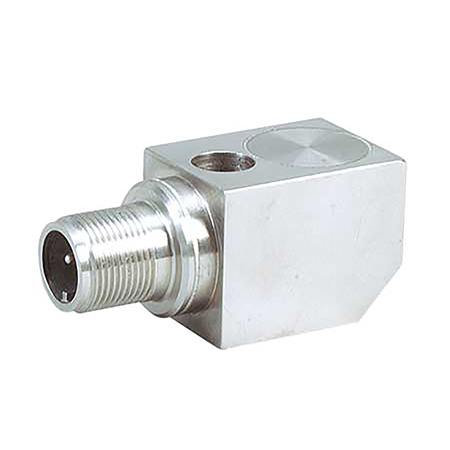
\includegraphics[width=0.3\textwidth]{acelerometro.jpg}
	\caption{Acelerómetro con salida lateral industrial de uso general}
\end{figure}

